 

\begin{enumerate}[label=(\arabic*),leftmargin=0.7cm]

\item Size properties of our multiscale test $\mathcal{T}_{\text{MS}}$.

\begin{table}[h!]
\footnotesize{
\caption{Size of $\mathcal{T}_{\text{MS}}$ for different AR parameters $a_1$, sample sizes $T$ and nominal sizes $\alpha$ for the estimated long-run variance.}
\newcolumntype{C}[1]{>{\hsize=#1\hsize\centering\arraybackslash}X}
\newcolumntype{Z}{>{\centering\arraybackslash}X}
\begin{tabularx}{\textwidth}{C{3} C{0.01} ZZZ C{0.01} ZZZ C{0.01} ZZZ C{0.01} ZZZ} 
\toprule
 & &  \multicolumn{3}{c}{$a_1 = -0.5$} & &  \multicolumn{3}{c}{$a_1 = -0.25$} & &  \multicolumn{3}{c}{$a_1 = 0.25$}  & &  \multicolumn{3}{c}{$a_1 = 0.5$} \\
\cmidrule[0.4pt]{3-5} \cmidrule[0.4pt]{7-9} \cmidrule[0.4pt]{11-13} \cmidrule[0.4pt]{15-17} 
 & &  \multicolumn{3}{c}{nominal size $\alpha$} & &  \multicolumn{3}{c}{nominal size $\alpha$} & &  \multicolumn{3}{c}{nominal size $\alpha$} & &  \multicolumn{3}{c}{nominal size $\alpha$} \\
 & &  0.01 & 0.05 & 0.1   & &  0.01 & 0.05 & 0.1   & &  0.01 & 0.05 & 0.1  & &  0.01 & 0.05 & 0.1   \\
\cmidrule[0.4pt]{1-17}
$T = 250$ &  & 0.015 & 0.049 & 0.117 &  & 0.009 & 0.052 & 0.111 &  & 0.013 & 0.047 & 0.110 &  & 0.017 & 0.048 & 0.109 \\ 
$T =   500$ &  & 0.008 & 0.056 & 0.128 &  & 0.017 & 0.047 & 0.112 &  & 0.014 & 0.050 & 0.100 &  & 0.014 & 0.048 & 0.107 \\ 
$T =   1000$ &  & 0.007 & 0.053 & 0.090 &  & 0.014 & 0.059 & 0.106 &  & 0.014 & 0.056 & 0.099 &  & 0.017 & 0.057 & 0.099 \\ 
\bottomrule
\end{tabularx}}
\end{table}

\begin{table}[h!]
\footnotesize{
\caption{Size of $\mathcal{T}_{\text{MS}}$ for different AR parameters $a_1$, sample sizes $T$ and nominal sizes $\alpha$ for the true long-run variance.}
\newcolumntype{C}[1]{>{\hsize=#1\hsize\centering\arraybackslash}X}
\newcolumntype{Z}{>{\centering\arraybackslash}X}
\begin{tabularx}{\textwidth}{C{3} C{0.01} ZZZ C{0.01} ZZZ C{0.01} ZZZ C{0.01} ZZZ} 
\toprule
 & &  \multicolumn{3}{c}{$a_1 = -0.5$} & &  \multicolumn{3}{c}{$a_1 = -0.25$} & &  \multicolumn{3}{c}{$a_1 = 0.25$}  & &  \multicolumn{3}{c}{$a_1 = 0.5$} \\
 \cmidrule[0.4pt]{3-5} \cmidrule[0.4pt]{7-9} \cmidrule[0.4pt]{11-13}  \cmidrule[0.4pt]{15-17} 
 & &  \multicolumn{3}{c}{nominal size $\alpha$} & &  \multicolumn{3}{c}{nominal size $\alpha$} & &  \multicolumn{3}{c}{nominal size $\alpha$} & &  \multicolumn{3}{c}{nominal size $\alpha$} \\
 & &  0.01 & 0.05 & 0.1   & &  0.01 & 0.05 & 0.1   & &  0.01 & 0.05 & 0.1  & &  0.01 & 0.05 & 0.1   \\
\cmidrule[0.4pt]{1-17}
$T = 250$ &  & 0.014 & 0.053 & 0.107 &  & 0.013 & 0.049 & 0.104 &  & 0.014 & 0.046 & 0.093 &  & 0.011 & 0.043 & 0.082 \\ 
$T =   500$ &  & 0.014 & 0.049 & 0.103 &  & 0.014 & 0.049 & 0.099 &  & 0.014 & 0.047 & 0.096 &  & 0.013 & 0.044 & 0.091 \\ 
$T =   1000$ &  & 0.010 & 0.050 & 0.105 &  & 0.010 & 0.050 & 0.107 &  & 0.010 & 0.044 & 0.105 &  & 0.009 & 0.043 & 0.097 \\ 
\bottomrule
\end{tabularx}}
\end{table}

\begin{table}[h!]
\footnotesize{
\caption{Size of $\mathcal{T}_{\text{MS}}$ for different AR parameters $a_1$, sample sizes $T$ and nominal sizes $\alpha$ for the estimated long-run variance.}
\newcolumntype{C}[1]{>{\hsize=#1\hsize\centering\arraybackslash}X}
\newcolumntype{Z}{>{\centering\arraybackslash}X}
\begin{tabularx}{\textwidth}{C{3} C{0.01} ZZZZZZZ C{0.01} ZZZZZZZ} 
\toprule
 & &  \multicolumn{7}{c}{$a_1 = -0.9$} & &  \multicolumn{7}{c}{$a_1 = 0.9$} \\
\cmidrule[0.4pt]{3-9} \cmidrule[0.4pt]{11-17}  
 & &  \multicolumn{7}{c}{sample size $T$} & &  \multicolumn{7}{c}{sample size $T$} \\
 & &  250 & 500 & 1000 &2000 &3000 &4000 &5000  & &  250 & 500 & 1000 &2000 &3000 &4000 &5000 \\
\cmidrule[0.4pt]{1-17}
 $\alpha = 0.01$ &  & 0.057 & 0.033 & 0.032 & 0.014 & 0.011 & 0.018 & 0.011 &  & 0.004 & 0.012 & 0.023 & 0.015 & 0.019 & 0.019 & 0.020 \\ 
 $\alpha =  0.05$ &  & 0.134 & 0.098 & 0.091 & 0.055 & 0.046 & 0.057 & 0.049 &  & 0.016 & 0.040 & 0.076 & 0.062 & 0.050 & 0.057 & 0.060 \\ 
$\alpha =   0.1$ &  & 0.233 & 0.193 & 0.156 & 0.109 & 0.103 & 0.108 & 0.095 &  & 0.039 & 0.079 & 0.103 & 0.120 & 0.116 & 0.111 & 0.113 \\ 

\bottomrule
\end{tabularx}}
\end{table}

\begin{table}[h!]
\footnotesize{
\caption{Size of $\mathcal{T}_{\text{MS}}$ for different AR parameters $a_1$, sample sizes $T$ and nominal sizes $\alpha$ for the true long-run variance.}
\newcolumntype{C}[1]{>{\hsize=#1\hsize\centering\arraybackslash}X}
\newcolumntype{Z}{>{\centering\arraybackslash}X}
\begin{tabularx}{\textwidth}{C{3} C{0.01} ZZZZZZZ C{0.01} ZZZZZZZ} 
\toprule
 & &  \multicolumn{7}{c}{$a_1 = -0.9$} & &  \multicolumn{7}{c}{$a_1 = 0.9$} \\
\cmidrule[0.4pt]{3-9} \cmidrule[0.4pt]{11-17}  
 & &  \multicolumn{7}{c}{sample size $T$} & &  \multicolumn{7}{c}{sample size $T$} \\
 & &  250 & 500 & 1000 &2000 &3000 &4000 &5000  & &  250 & 500 & 1000 &2000 &3000 &4000 &5000 \\
\cmidrule[0.4pt]{1-17}
$\alpha =  0.01$ &  & 0.058 & 0.036 & 0.027 & 0.014 & 0.010 & 0.016 & 0.011 &  & 0.003 & 0.005 & 0.005 & 0.008 & 0.009 & 0.008 & 0.009 \\ 
$\alpha =   0.05 $&  & 0.136 & 0.092 & 0.090 & 0.056 & 0.048 & 0.056 & 0.048 &  & 0.010 & 0.019 & 0.028 & 0.036 & 0.042 & 0.046 & 0.040 \\ 
$\alpha =   0.1$ &  & 0.231 & 0.196 & 0.154 & 0.109 & 0.107 & 0.107 & 0.103 &  & 0.024 & 0.044 & 0.053 & 0.068 & 0.087 & 0.093 & 0.090 \\ 
\bottomrule
\end{tabularx}}
\end{table}

\begin{table}[h!]
\footnotesize{
\caption{Size of $\mathcal{T}_{\text{MS}}$ for different AR parameters $a_1$, sample sizes $T$ and nominal sizes $\alpha$ for the true long-run variance.}
\newcolumntype{C}[1]{>{\hsize=#1\hsize\centering\arraybackslash}X}
\newcolumntype{Z}{>{\centering\arraybackslash}X}
\begin{tabularx}{\textwidth}{C{3} C{0.01} ZZZZ C{0.01} ZZZZ} 
\toprule
 & &  \multicolumn{4}{c}{$a_1 = -0.5$} & &  \multicolumn{4}{c}{$a_1 = 0.5$} \\
\cmidrule[0.4pt]{3-6} \cmidrule[0.4pt]{8-11}  
& &  $\mathcal{T}_{\text{MS}}$ & $\mathcal{T}_{\text{uncor}}$ &  $\mathcal{T}_{\text{rows}}$ & $ \mathcal{T}_{\text{SiZer}}$ & &  $\mathcal{T}_{\text{MS}}$ & $\mathcal{T}_{\text{uncor}}$ & $ \mathcal{T}_{\text{rows}}$ & $ \mathcal{T}_{\text{SiZer}}$\\
\cmidrule[0.4pt]{1-11}
$T=250$ &  & 0.064 & 0.080 & 0.305 & 0.379 &  & 0.050 & 0.037 & 0.121 & 0.310 \\ 
 $T =  500$ &  & 0.055 & 0.072 & 0.351 & 0.445 &  & 0.047 & 0.042 & 0.180 & 0.394 \\ 
 $T = 1000$ &  & 0.059 & 0.076 & 0.413 & 0.552 &  & 0.046 & 0.042 & 0.232 & 0.491 \\ 
\bottomrule
\end{tabularx}}
\end{table}

\item Comparison of the multiscale test $\mathcal{T}_{\text{MS}}$ with its uncorrected version $\mathcal{T}_{\text{UC}}$, its row-wise version $\mathcal{T}_{\text{RW}}$ and (row-wise) SiZer $\mathcal{T}_{\text{SiZer}}$. 

For the comparison, we focus on the significance level $\alpha=0.05$ and on the AR parameters $a_1 \in \{-0.5,0.5\}$. (Maybe report results for other AR parameters and significance levels in supplement?)


\begin{figure}[t]
\begin{subfigure}{.5\textwidth}
\centering
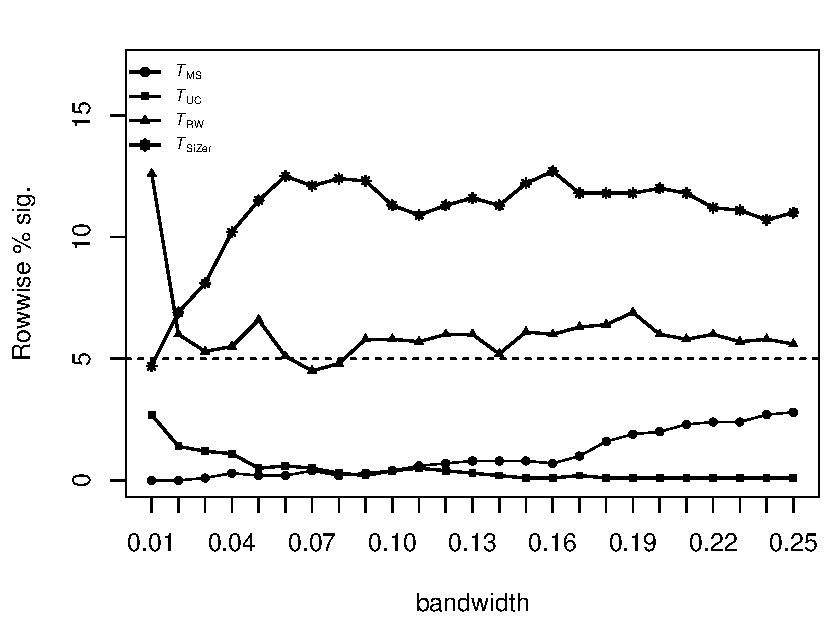
\includegraphics[width=.9\linewidth]{Plots/pcp_rowwise_T_500_a1_-50.pdf}
\caption{$a_1 = -0.50$}
\end{subfigure}
\begin{subfigure}{.5\textwidth}
\centering
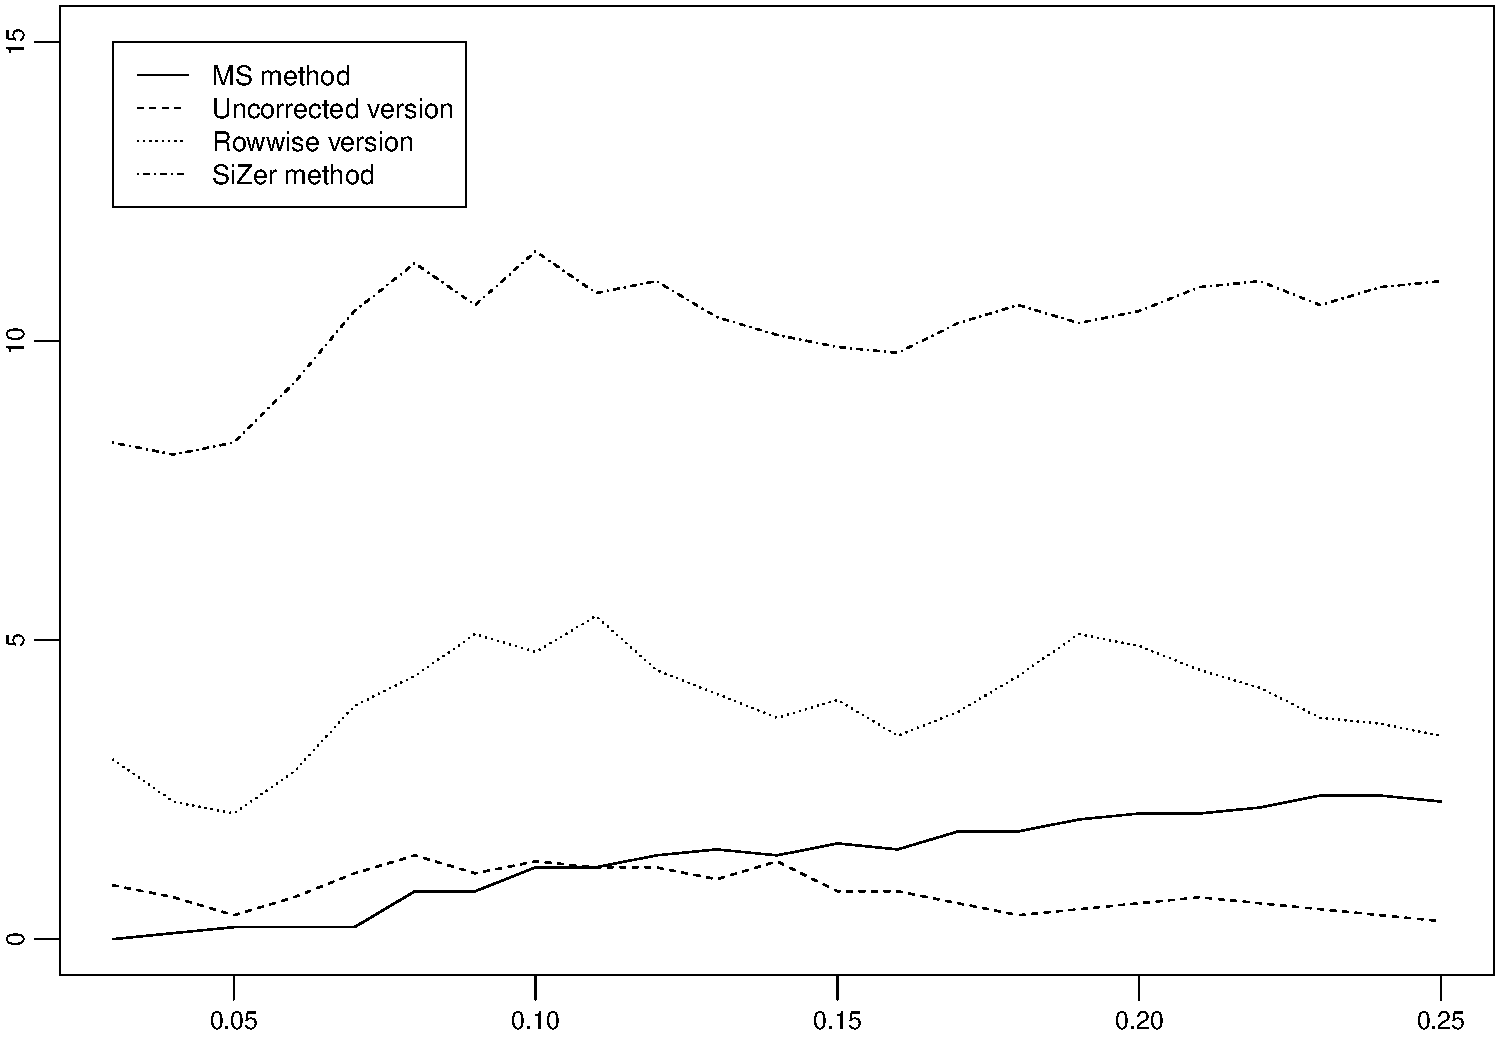
\includegraphics[width=.9\linewidth]{Plots/pcp_rowwise_T_500_a1_50.pdf}
\caption{$a_1 = 0.50$}
\end{subfigure}
\caption{Rowwise power comparison}  
\label{fig:comparison_rowwise_size}
\end{figure}

\begin{enumerate}[label=(\alph*),leftmargin=0.7cm]

\item Size comparisons:
\begin{itemize}[label=--,leftmargin=0.5cm]
\item Comparison of global size (as in Figure 6 of Hannig \& Marron (2006)).
\item Comparison of row-wise size (as in Figure 7 of Hannig \& Marron (2006)). (Three plots, each corresponding to one sample size $T=250, 500, 1000$. Or one plot for all three sample sizes? Too packed?)  
\end{itemize}

\item Power comparisons: 
\begin{itemize}[label=--,leftmargin=0.5cm]
%\item We first consider two simple signals. I think we may stick with the two types of signals that we had in the old Section 7.2 (Comparison with SiZer): 
%(i) a global signal: a linear trend $m(u) = \beta (u - 0.5)$ with ONE slope $\beta$ which may be different for $a_1 = -0.5$ and $a_1 = 0.5$. 
%(ii) a local signal: the bump function $m(u) = 0.5 \cdot \ind(u \in [0.45,0.55]) \cdot (1 - \{\frac{(u-0.5}{0.05}\}^2)^2$. (This is the same bump function as in Section 7.2, but more localized and smaller, so that it is harder to detect.)
\item We first consider a version of the bump signal that we already had in the old Section 7.2 (Comparison with SiZer): $m(u) = 0.5 \cdot \ind(u \in [0.45,0.55]) \cdot (1 - \{\frac{(u-0.5}{0.05}\}^2)^2$. (This is the same bump function as in Section 7.2, but more localized and smaller, so that it is harder to detect.) \\[0.1cm]
Set $T=500$. We make the following power comparisons for the bump signal: \\[0.1cm]
(i) comparison of global power and global spurious power reported in a table of the same form as Table \ref{tab:bump_power_spuriouspower}. 

\begin{table}[h!]
\centering
\footnotesize{
\caption{Global power comparison for the bump signal}\label{tab:bump_power_spuriouspower}
\newcolumntype{C}[1]{>{\hsize=#1\hsize\centering\arraybackslash}X}
\newcolumntype{Z}{>{\centering\arraybackslash}X}
\begin{tabularx}{\textwidth}{C{3} C{0.0001} ZZZZ C{0.0001} ZZZZ} 
\toprule
%        & & \multicolumn{6}{c}{$a_1 = -0.25$} & & \multicolumn{6}{c}{$a_1 = 0.25$} \\ 
%\cmidrule[0.4pt]{3-8} \cmidrule[0.4pt]{10-15}
        & & \multicolumn{4}{c}{$a_1=-0.5$} & & \multicolumn{4}{c}{$a_1=0.5$} \\[0.1cm]
        & & $\mathcal{T}_{\text{MS}}$ & $\mathcal{T}_{\text{UC}}$ & $\mathcal{T}_{\text{RW}}$ & $\mathcal{T}_{\text{SiZer}}$ & & $\mathcal{T}_{\text{MS}}$ & $\mathcal{T}_{\text{UC}}$ & $\mathcal{T}_{\text{RW}}$ & $\mathcal{T}_{\text{SiZer}}$ \\
\cmidrule[0.4pt]{1-11}
Power  & & 0.000 & 0.000 & 0.000 & 0.000 & & 0.000 & 0.000 & 0.000 & 0.000 \\ 
Spurious power & & 0.000 & 0.000 & 0.000 & 0.000 & & 0.000 & 0.000 & 0.000 & 0.000 \\ 
\bottomrule
\end{tabularx}}
\end{table}

(ii) comparison of rowwise power reported in a plot of the same format as Figure 7 of Hannig \& Marron (2006) / Figure \ref{fig:bump-power} below. 

\begin{figure}[h!]
\centering
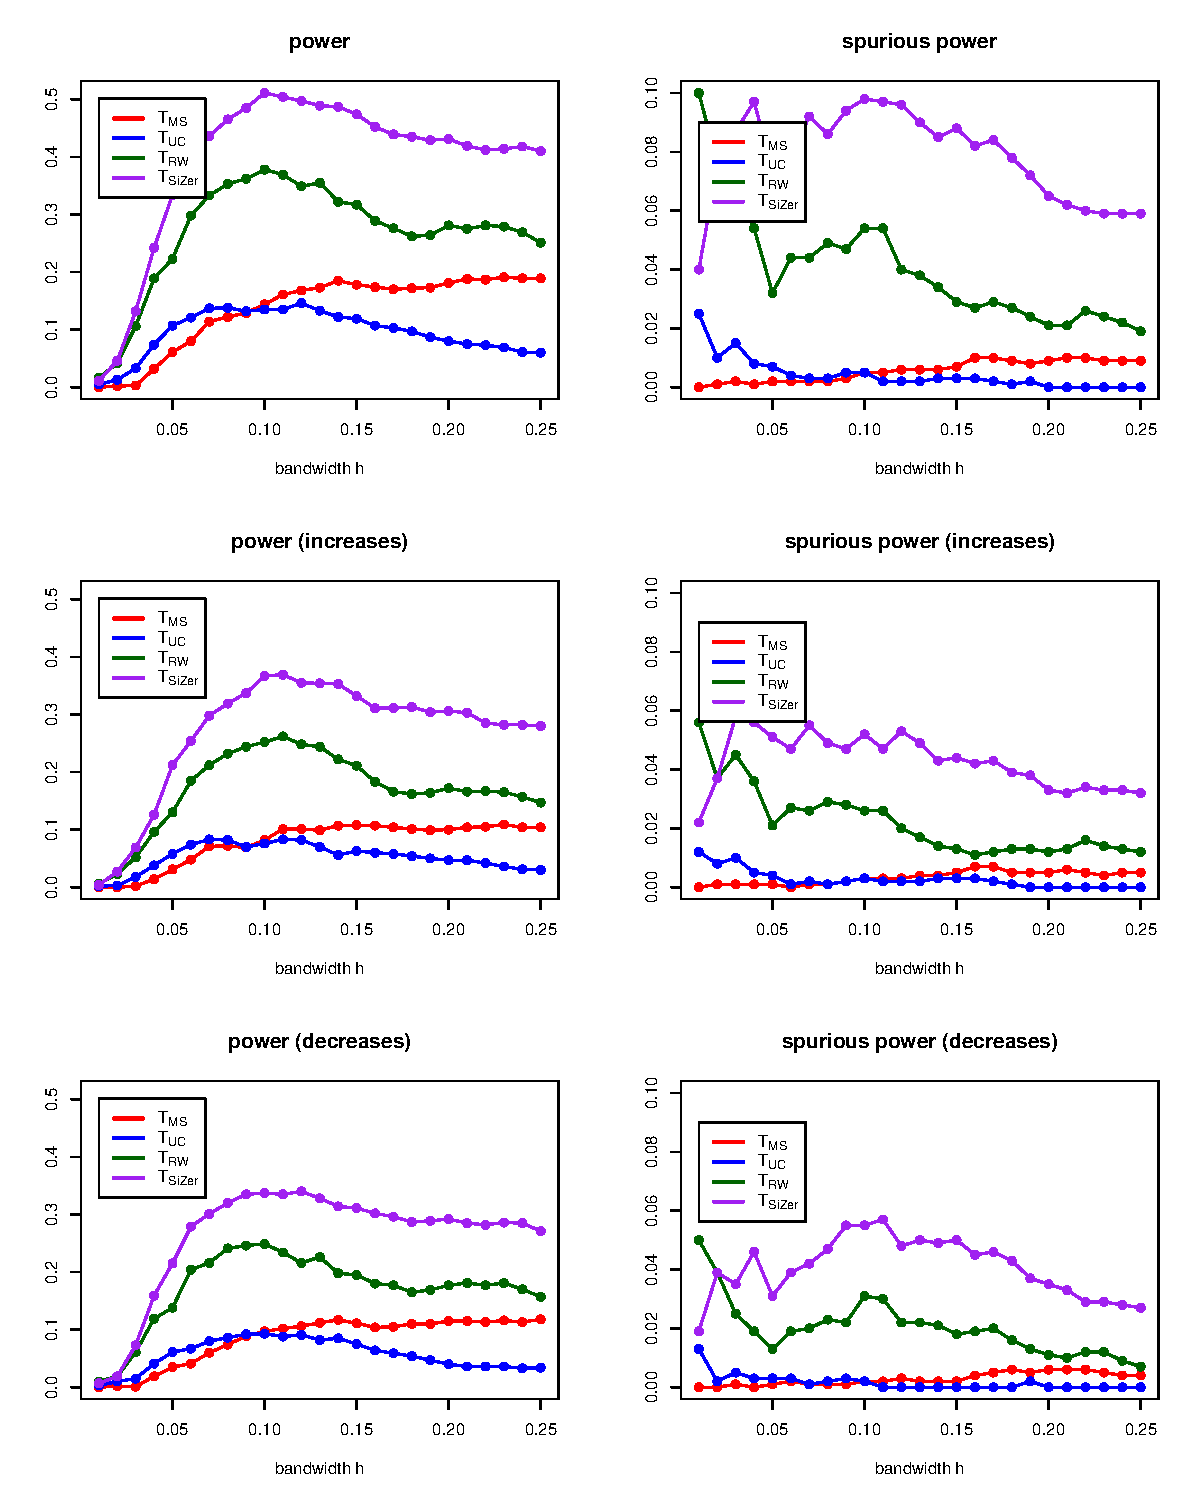
\includegraphics[width=0.7\textwidth]{Plots/power_comparison.pdf}
\caption{Rowwise power comparison for bump signal.}\label{fig:bump-power}
\end{figure}
\end{itemize}

\item Power comparisons by means of ``more interesting'' signals (e.g.\ the blocks signal of Donoho): plot of SiZer maps and minimal intervals. 


\end{enumerate}
\end{enumerate}

\FloatBarrier



\subsection{Size and power properties of the multiscale test}\label{subsec-sim-1} 


Our simulation design mimics the situation in the application example of Section \ref{sec-data}. We generate data from the model $Y_{t,T} = m(t/T) + \varepsilon_t$ for different trend functions $m$, error processes $\{\varepsilon_t\}$ and time series lengths $T$. The error terms are supposed to have the AR($1$) structure $\varepsilon_t = a_1 \varepsilon_{t-1} + \eta_t$, where $a_1 \in \{-0.5,-0.25,0.25,0.5\}$ and $\eta_t$ are i.i.d.\ standard normal. In addition, we consider the AR($2$) specification $\varepsilon_t = a_1 \varepsilon_{t-1} + a_2 \varepsilon_{t-2} + \eta_t$, where $\eta_t$ are normally distributed with $\ex[\eta_t] = 0$ and $\ex[\eta_t^2] = \nu^2$. We set $a_1 = 0.167$, $a_2 = 0.178$ and $\nu^2 = 0.322$, thus matching the estimated values obtained in the application of Section \ref{sec-data}. To simulate data under the null hypothesis, we let $m$ be a constant function. In particular, we set $m = 0$ without loss of generality. To generate data under the alternative, we consider the trend functions $m(u) = \beta (u - 0.5) \cdot \ind(0.5 \le u \le 1)$ with $\beta = 1.5,2.0,2.5$. These functions are broken lines with a kink at $u = 0.5$ and different slopes $\beta$. Their shape roughly resembles the trend estimates in the application of Section \ref{sec-data}. The slope parameter $\beta$ corresponds to a trend with the value $m(1) = 0.5 \beta$ at the right endpoint $u = 1$. We thus consider broken lines with the values $m(1) = 0.75, 1.0, 1.25$. Inspecting the middle panel of Figure \ref{plot-results-app1}, the broken lines with the endpoints $m(1) = 1.0$ and $m(1) = 1.25$ (that is, with $\beta = 2.0$ and $\beta = 2.5$) can be seen to resemble the local linear trend estimates in the real-data example the most (where we neglect the nonlinearities of the local linear fits at the beginning of the observation period). The broken line with $\beta = 1.5$ is closer to the null, making it harder for our test to detect this alternative.\footnote{The broken lines $m$ are obviously non-differentiable at the kink point. We could replace them by slightly smoothed versions to satisfy the differentiability assumption that is imposed in the theoretical part of the paper. However, as this leaves the simulation results essentially unchanged but only creates additional notation, we stick to the broken lines.}


%To simulate data under the null, we let $m$ be a constant function. In parti\-cular, we set $m = 0$ without loss of generality. To generate data under the alternative, we consider trend functions of the form $m(u) = \beta \cdot (u - 0.5) \cdot \ind(0.5 \le u \le 1)$ with the slope parameter $\beta$. These functions are broken lines with a kink at $u = 0.5$. Their shape roughly resembles the trend estimates in the application of Section \ref{sec-data}. For each AR specification of the errors, we consider three different slopes $\beta = s_\beta \cdot \sigma$ with $s_\beta \in \{1.7,2.3,2.9\}$ and $\sigma^2$ being the long-run error variance. The parameter $s_\beta$ is closely related to the signal-to-noise ratio in the model $Y_{t,T} = m(t/T) + \varepsilon_t$: The larger $s_\beta$, the stronger is the trend $m$ compared to the long-run error variance $\sigma^2$. The values $s_\beta \in \{ 1.7, 2.3, 2.9\}$ are motivated by the application example in Section \ref{sec-data}: For the AR($2$) specification which mimics the data example, it holds that $\beta \approx 1.5, 2.0, 2.5$ for $s_\beta = 1.7,2.3,2.9$. As the slope parameter $\beta$ corresponds to a trend with the value $m(1) = 0.5 \cdot \beta$ at the right endpoint $u = 1$, we thus consider broken lines with the values $m(1) \approx 0.75, 1.0, 1.25$ in this case. Inspecting the middle panel of Figure \ref{plot-results-app1}, the broken lines with the endpoints $m(1) \approx 1.0$ and $m(1) \approx 1.25$ (that is, with $s_\beta = 2.3$ and $s_\beta = 2.9$) can be seen to resemble the local linear trend estimates in the real-data example the most (where we neglect the nonlinearities of the local linear fits at the beginning of the observation period). The broken line with $s_\beta = 1.7$ has a smaller slope $\beta$ and is thus closer to the null, making it harder for our test to detect this alternative.\footnote{The broken lines $m$ are obviously non-differentiable at the kink point. We could replace them by slightly smoothed versions to satisfy the differentiability assumption that is imposed in the theoretical part of the paper. However, as this leaves the simulation results essentially unchanged but only creates additional notation, we stick to the broken lines.}


\begin{sidewaystable}
\centering
\footnotesize{
\caption{Size of our multiscale test for different AR parameters $a_1$ and $a_2$, sample sizes $T$ and nominal sizes $\alpha$.}\label{tab:size_test}
\newcolumntype{C}[1]{>{\hsize=#1\hsize\centering\arraybackslash}X}
\newcolumntype{Z}{>{\centering\arraybackslash}X}
\begin{tabularx}{\textwidth}{C{2} C{0.1} ZZZ C{0.1} ZZZ C{0.1} ZZZ C{0.1} ZZZ C{0.1} ZZZ} 
\toprule
 & &  \multicolumn{3}{c}{$a_1 = -0.5$} & &  \multicolumn{3}{c}{$a_1 = -0.25$} & &  \multicolumn{3}{c}{$a_1 = 0.25$} & &  \multicolumn{3}{c}{$a_1 = 0.5$} & &  \multicolumn{3}{c}{$(a_1,a_2) = (0.167,0.178)$} \\
\cmidrule[0.4pt]{3-5} \cmidrule[0.4pt]{7-9} \cmidrule[0.4pt]{11-13} \cmidrule[0.4pt]{15-17} \cmidrule[0.4pt]{19-21}
 & &  \multicolumn{3}{c}{nominal size $\alpha$} & &  \multicolumn{3}{c}{nominal size $\alpha$} & &  \multicolumn{3}{c}{nominal size $\alpha$} & &  \multicolumn{3}{c}{nominal size $\alpha$} & &  \multicolumn{3}{c}{nominal size $\alpha$} \\
 & &  0.01 & 0.05  & 0.1 & &  0.01 & 0.05  & 0.1  & &  0.01 & 0.05  & 0.1  & &  0.01 & 0.05  & 0.1  & &  0.01 & 0.05  & 0.1   \\
\cmidrule[0.4pt]{1-21}
$T = 250$ &  & 0.015 & 0.050 & 0.127 &  & 0.014 & 0.057 & 0.120 &  & 0.011 & 0.046 & 0.116 &  & 0.013 & 0.042 & 0.108 &  & 0.011 & 0.052 & 0.117 \\ 
 $T= 350$ &  & 0.009 & 0.067 & 0.120 &  & 0.010 & 0.055 & 0.095 &  & 0.009 & 0.055 & 0.096 &  & 0.010 & 0.049 & 0.090 &  & 0.010 & 0.059 & 0.114 \\ 
 $T= 500$ &  & 0.015 & 0.053 & 0.128 &  & 0.015 & 0.047 & 0.100 &  & 0.018 & 0.048 & 0.101 &  & 0.015 & 0.042 & 0.106 &  & 0.015 & 0.056 & 0.107 \\ 
\bottomrule
\end{tabularx}
\vspace{0.5cm}

\caption{Power of our multiscale test for different AR parameters $a_1$ and $a_2$, sample sizes $T$ and nominal sizes $\alpha$. The three panels (a)--(c) corresponds to different slope parameters $\beta$ of the broken line $m$.}\label{tab:power_test}

\begin{tabularx}{\textwidth}{C{2} C{0.1} ZZZ C{0.1} ZZZ C{0.1} ZZZ C{0.1} ZZZ C{0.1} ZZZ} 
\multicolumn{21}{c}{(a) $\beta = 1.5$} \\[0.2cm]
\toprule
 & &  \multicolumn{3}{c}{$a_1 = -0.5$} & &  \multicolumn{3}{c}{$a_1 = -0.25$} & &  \multicolumn{3}{c}{$a_1 = 0.25$} & &  \multicolumn{3}{c}{$a_1 = 0.5$} & &  \multicolumn{3}{c}{$(a_1,a_2) = (0.167,0.178)$} \\
\cmidrule[0.4pt]{3-5} \cmidrule[0.4pt]{7-9} \cmidrule[0.4pt]{11-13} \cmidrule[0.4pt]{15-17} \cmidrule[0.4pt]{19-21}
 & &  \multicolumn{3}{c}{nominal size $\alpha$} & &  \multicolumn{3}{c}{nominal size $\alpha$} & &  \multicolumn{3}{c}{nominal size $\alpha$} & &  \multicolumn{3}{c}{nominal size $\alpha$} & &  \multicolumn{3}{c}{nominal size $\alpha$} \\
 & &  0.01 & 0.05  & 0.1   & &  0.01 & 0.05  & 0.1   & &  0.01 & 0.05  & 0.1    & &  0.01 & 0.05  & 0.1    & &  0.01 & 0.05  & 0.1   \\
\cmidrule[0.4pt]{1-21}
$T=250$ &  & 0.484 & 0.726 & 0.853 &  & 0.319 & 0.548 & 0.702 &  & 0.077 & 0.177 & 0.324 &  & 0.036 & 0.097 & 0.181 &  & 0.269 & 0.460 & 0.612 \\ 
 $T= 350$ &  & 0.735 & 0.913 & 0.955 &  & 0.463 & 0.753 & 0.834 &  & 0.116 & 0.273 & 0.385 &  & 0.050 & 0.141 & 0.221 &  & 0.390 & 0.654 & 0.770 \\ 
  $T=500$ &  & 0.945 & 0.988 & 0.997 &  & 0.775 & 0.925 & 0.972 &  & 0.195 & 0.389 & 0.551 &  & 0.060 & 0.162 & 0.285 &  & 0.623 & 0.815 & 0.907 \\ 
\bottomrule
\end{tabularx}
\vspace{0.25cm}

\begin{tabularx}{\textwidth}{C{2} C{0.1} ZZZ C{0.1} ZZZ C{0.1} ZZZ C{0.1} ZZZ C{0.1} ZZZ} 
\multicolumn{21}{c}{(b) $\beta = 2.0$} \\[0.2cm]
\toprule
 & &  \multicolumn{3}{c}{$a_1 = -0.5$} & &  \multicolumn{3}{c}{$a_1 = -0.25$} & &  \multicolumn{3}{c}{$a_1 = 0.25$} & &  \multicolumn{3}{c}{$a_1 = 0.5$} & &  \multicolumn{3}{c}{$(a_1,a_2) = (0.167,0.178)$} \\
\cmidrule[0.4pt]{3-5} \cmidrule[0.4pt]{7-9} \cmidrule[0.4pt]{11-13} \cmidrule[0.4pt]{15-17} \cmidrule[0.4pt]{19-21}
 & &  \multicolumn{3}{c}{nominal size $\alpha$} & &  \multicolumn{3}{c}{nominal size $\alpha$} & &  \multicolumn{3}{c}{nominal size $\alpha$} & &  \multicolumn{3}{c}{nominal size $\alpha$} & &  \multicolumn{3}{c}{nominal size $\alpha$} \\
 & &  0.01 & 0.05  & 0.1   & &  0.01 & 0.05  & 0.1   & &  0.01 & 0.05  & 0.1    & &  0.01 & 0.05  & 0.1    & &  0.01 & 0.05  & 0.1   \\
\cmidrule[0.4pt]{1-21}
$T = 250$ &  & 0.869 & 0.961 & 0.985 &  & 0.663 & 0.846 & 0.916 &  & 0.164 & 0.340 & 0.520 &  & 0.062 & 0.143 & 0.259 &  & 0.549 & 0.724 & 0.851 \\ 
$T=  350$ &  & 0.979 & 0.997 & 1.000 &  & 0.863 & 0.969 & 0.986 &  & 0.262 & 0.483 & 0.615 &  & 0.092 & 0.231 & 0.334 &  & 0.759 & 0.922 & 0.958 \\ 
 $T= 500$ &  & 1.000 & 1.000 & 1.000 &  & 0.983 & 0.997 & 0.999 &  & 0.469 & 0.716 & 0.821 &  & 0.137 & 0.309 & 0.451 &  & 0.933 & 0.983 & 0.994 \\ 
\bottomrule
\end{tabularx}
\vspace{0.25cm}

\begin{tabularx}{\textwidth}{C{2} C{0.1} ZZZ C{0.1} ZZZ C{0.1} ZZZ C{0.1} ZZZ C{0.1} ZZZ} 
\multicolumn{21}{c}{(c) $\beta = 2.5$} \\[0.2cm]
\toprule
 & &  \multicolumn{3}{c}{$a_1 = -0.5$} & &  \multicolumn{3}{c}{$a_1 = -0.25$} & &  \multicolumn{3}{c}{$a_1 = 0.25$} & &  \multicolumn{3}{c}{$a_1 = 0.5$} & &  \multicolumn{3}{c}{$(a_1,a_2) = (0.167,0.178)$} \\
\cmidrule[0.4pt]{3-5} \cmidrule[0.4pt]{7-9} \cmidrule[0.4pt]{11-13} \cmidrule[0.4pt]{15-17} \cmidrule[0.4pt]{19-21}
 & &  \multicolumn{3}{c}{nominal size $\alpha$} & &  \multicolumn{3}{c}{nominal size $\alpha$} & &  \multicolumn{3}{c}{nominal size $\alpha$} & &  \multicolumn{3}{c}{nominal size $\alpha$} & &  \multicolumn{3}{c}{nominal size $\alpha$} \\
 & &  0.01 & 0.05  & 0.1   & &  0.01 & 0.05  & 0.1   & &  0.01 & 0.05  & 0.1    & &  0.01 & 0.05  & 0.1    & &  0.01 & 0.05  & 0.1   \\
\cmidrule[0.4pt]{1-21}
$T=250$ &  & 0.989 & 1.000 & 1.000 &  & 0.901 & 0.971 & 0.993 &  & 0.322 & 0.543 & 0.703 &  & 0.100 & 0.224 & 0.367 &  & 0.804 & 0.918 & 0.958 \\ 
 $T= 350$ &  & 1.000 & 1.000 & 1.000 &  & 0.990 & 1.000 & 1.000 &  & 0.470 & 0.737 & 0.833 &  & 0.162 & 0.361 & 0.481 &  & 0.950 & 0.988 & 0.997 \\ 
 $T= 500$ &  & 1.000 & 1.000 & 1.000 &  & 0.999 & 1.000 & 1.000 &  & 0.773 & 0.919 & 0.968 &  & 0.285 & 0.473 & 0.649 &  & 0.994 & 0.999 & 1.000 \\ 
\bottomrule
\end{tabularx}
}
\end{sidewaystable}


To implement our test, we choose $K$ to be an Epanechnikov kernel and define the set $\mathcal{G}_T$ of location-scale points $(u,h)$ as
\begin{align}
\mathcal{G}_T = \big\{ (u, h): & \, \, u = 5k/T \text{ for some } 1 \le k \le T/5 \text{ and } \nonumber \\ & \, \, h = (3+5\ell)/T \text{ for some } 0 \le \ell \le T/20 \big\}. \label{grid-sim-app}
\end{align}
We thus take into account all rescaled time points $u \in [0,1]$ on an equidistant grid with step length $5/T$. For the bandwidth $h = (3 + 5\ell)/T$ and any $u \in [h,1-h]$, the kernel weights $\kernel(h^{-1} \{t/T-u\})$ are non-zero for exactly $5 + 10 \ell$ observations. Hence, the bandwidths $h$ in $\mathcal{G}_T$ correspond to effective sample sizes of $5, 15, 25, \ldots$ up to approximately $T/4$ data points. As a robustness check, we have re-run the simulations for a number of other grids. As the results are very similar, we do however not report them here. The long-run error variance $\sigma^2$ is estimated by the procedures from Section \ref{subsec-error-var-AR}: We first compute the estimator $\widehat{\boldsymbol{a}}$ of the AR parameter(s), where we use $\overline{r} = 10$ and the pilot estimator $\widetilde{\boldsymbol{a}}_q$ with $q = 25$. Based on $\widehat{\boldsymbol{a}}$, we then compute the estimator $\widehat{\sigma}^2$ of the long-run error variance $\sigma^2$. As a further robustness check, we have re-run the simulations for other choices of the parameters $q$ and $\overline{r}$, which yields very similar results. The dependence of the estimators $\widehat{\boldsymbol{a}}$ and $\widehat{\sigma}^2$ on $q$ and $\overline{r}$ is further explored in Section \ref{subsec-sim-3}. To compute the critical values of the multiscale test, we simulate $1000$ values of the statistic $\Phi_T$ defined in Section \ref{subsec-method-test} and compute their empirical $(1-\alpha)$ quantile $q_T(\alpha)$. 


Tables \ref{tab:size_test} and \ref{tab:power_test} report the simulation results for the sample sizes $T=250,350,500$ and the significance levels $\alpha = 0.01, 0.05, 0.10$. The sample size $T = 350$ is approximately equal to the time series length $359$ in the real-data example of Section \ref{sec-data}. To produce our simulation results, we generate $S=1000$ samples for each model specification and carry out the multiscale test for each sample. The entries of Tables \ref{tab:size_test} and \ref{tab:power_test} are computed as the number of simulations in which the test rejects divided by the total number of simulations. As can be seen from Table \ref{tab:size_test}, the actual size of the test is fairly close to the nominal target $\alpha$ for all the considered AR specifications and sample sizes. Hence, the test has approximately the correct size. Inspecting Table \ref{tab:power_test}, one can further see that the test has reasonable power properties. For all the considered AR specifications, the power increases quickly (i) as the sample size gets larger and (ii) as we move away from the null by increasing the slope parameter $\beta$. The power is of course quite different across the various AR specifications. In particular, it is much lower for positive than for negative values of $a_1$ in the AR($1$) case, the lowest power numbers being obtained for the largest positive value $a_1 = 0.5$ under consideration. This reflects the fact that it is more difficult to detect a trend when there is strong positive autocorrelation in the data. For the AR($2$) specification of the errors, the sample size $T=350$ and the slopes $\beta = 2.0$ and $\beta = 2.5$, which yield the two model specifications that resemble the real-life data in Section \ref{sec-data} the most, the power of the test is above $92\%$ for the significance levels $\alpha = 0.05$ and $\alpha = 0.1$ and above $75\%$ for $\alpha = 0.01$. Hence, our method has substantial power in the two simulation scenarios which are closest to the situation in the application. 


\subsection{Comparison with SiZer}\label{subsec-sim-2}


We now compare our multiscale test to SiZer for times series which was developed in \cite{Rondonotti2004}, \cite{Rondonotti2007} and \cite{ParkHannigKang2009}. Roughly speaking, the SiZer method proceeds as follows: For each location $u$ and bandwidth $h$ in a pre-specified set, SiZer computes an estimator $\widehat{m}_h^\prime(u)$ of the derivative $m^\prime(u)$ and a corresponding confidence interval. For each $(u,h)$, it then checks whether the confidence interval includes the value $0$. The set $\Pi_T^{\text{SiZer}}$ of points $(u,h)$ for which the confidence interval does not include $0$ corresponds to the set of intervals $\Pi_T^\pm$ for which our multiscale test finds an increase/decrease in the trend $m$. %rejects the null hypothesis $H_0$ that $m$ is constant on all intervals $[u-h,u+h]$ under consideration. 
In order to explore how our test performs in comparison to SiZer, we compare the two sets $\Pi_T^\pm$ and $\Pi_T^{\text{SiZer}}$ in different ways to each other in what follows. 


In order to implement SiZer for time series, we follow the exposition in \cite{ParkHannigKang2009}.\footnote{We have also examined the somewhat different implementation from \cite{Rondonotti2007}. As this yields worse simulation results than the procedure from \cite{ParkHannigKang2009}, we however do not report them here.} The details are given in Section S.3 in the Supplementary Material. To simplify the implementation of SiZer, we assume that the autocovariance function $\gamma_\varepsilon(\cdot)$ of the error process and thus the long-run error variance $\sigma^2$ is known. Our multiscale test is implemented in the same way as in Section \ref{subsec-sim-1}. To keep the comparison fair, we treat $\sigma^2$ as known also when implementing our method. Moreover, we use the same grid $\mathcal{G}_T$ of points $(u,h)$ for both methods. To achieve this, we start off with the grid $\mathcal{G}_T$ from \eqref{grid-sim-app}. We then follow \cite{Rondonotti2007} and \cite{ParkHannigKang2009} and restrict attention to those points $(u,h) \in \mathcal{G}_T$ for which the effective sample size $\text{ESS}^*(u,h)$ for correlated data is not smaller than $5$. This yields the grid $\mathcal{G}_T^* = \{ (u, h) \in \mathcal{G}_T : \text{ESS}^*(u, h) \geq 5 \}$. A detailed discussion of the effective sample size $\text{ESS}^*(u,h)$ for correlated data can be found in \cite{Rondonotti2007}.   


\begin{table}[t!]
\centering
\footnotesize{
\caption{Size of our multiscale test (MT) and SiZer for different model specifications.}\label{tab:size_comparison}
\newcolumntype{C}[1]{>{\hsize=#1\hsize\centering\arraybackslash}X}
\newcolumntype{Z}{>{\centering\arraybackslash}X}
\begin{tabularx}{\textwidth}{C{2} C{0.0001} ZZZZZZ C{0.0001} ZZZZZZ} 
\toprule
        & & \multicolumn{6}{c}{$a_1 = -0.25$} & & \multicolumn{6}{c}{$a_1 = 0.25$} \\ 
\cmidrule[0.4pt]{3-8} \cmidrule[0.4pt]{10-15}
        & & \multicolumn{2}{c}{$\alpha=0.01$} & \multicolumn{2}{c}{$\alpha=0.05$}  & \multicolumn{2}{c}{$\alpha=0.1$} 
        & & \multicolumn{2}{c}{$\alpha=0.01$} & \multicolumn{2}{c}{$\alpha=0.05$}  & \multicolumn{2}{c}{$\alpha=0.1$} \\[0.1cm]
        & & MT & SiZer & MT & SiZer & MT & SiZer & & MT & SiZer & MT & SiZer & MT & SiZer \\
\cmidrule[0.4pt]{1-15}
$T = 250$ &  & 0.018 & 0.112 & 0.040 & 0.374 & 0.104 & 0.575 &  & 0.017 & 0.106 & 0.034 & 0.347 & 0.092 & 0.522 \\ 
  $T= 350$ &  & 0.012 & 0.140 & 0.058 & 0.426 & 0.080 & 0.621 &  & 0.012 & 0.130 & 0.046 & 0.399 & 0.074 & 0.578 \\ 
  $T=500$ &  & 0.005 & 0.140 & 0.041 & 0.489 & 0.097 & 0.680 &  & 0.006 & 0.136 & 0.039 & 0.452 & 0.097 & 0.639 \\ 
\bottomrule
\end{tabularx}
\vspace{0.5cm}

\caption{Power of our multiscale test (MT) and SiZer for different model specifications. The three panels (a)--(c) corresponds to different slope parameters $\beta$ of the linear tend $m$.}\label{tab:power_comparison}
\newcolumntype{C}[1]{>{\hsize=#1\hsize\centering\arraybackslash}X}
\newcolumntype{Z}{>{\centering\arraybackslash}X}
\begin{tabularx}{\textwidth}{C{2} C{0.0001} ZZZZZZ C{0.0001} ZZZZZZ} 
\multicolumn{15}{c}{(a) $\beta = 1.0$ for negative $a_1$ and $\beta = 2.0$ for positive $a_1$} \\[0.2cm]
\toprule
        & & \multicolumn{6}{c}{$a_1 = -0.25$} & & \multicolumn{6}{c}{$a_1 = 0.25$} \\ 
\cmidrule[0.4pt]{3-8} \cmidrule[0.4pt]{10-15}
        & & \multicolumn{2}{c}{$\alpha=0.01$} & \multicolumn{2}{c}{$\alpha=0.05$}  & \multicolumn{2}{c}{$\alpha=0.1$} 
        & & \multicolumn{2}{c}{$\alpha=0.01$} & \multicolumn{2}{c}{$\alpha=0.05$}  & \multicolumn{2}{c}{$\alpha=0.1$} \\[0.1cm]
        & & MT & SiZer & MT & SiZer & MT & SiZer & & MT & SiZer & MT & SiZer & MT & SiZer \\
\cmidrule[0.4pt]{1-15}
$T = 250$ &  & 0.218 & 0.544 & 0.454 & 0.869 & 0.664 & 0.949 &  & 0.359 & 0.717 & 0.653 & 0.947 & 0.829 & 0.989 \\ 
 $T= 350$ &  & 0.385 & 0.707 & 0.665 & 0.958 & 0.753 & 0.986 &  & 0.599 & 0.888 & 0.864 & 0.995 & 0.913 & 0.998 \\ 
  $T=500$ &  & 0.581 & 0.899 & 0.862 & 0.993 & 0.949 & 0.999 &  & 0.851 & 0.981 & 0.983 & 1.000 & 0.999 & 1.000 \\ 
 \bottomrule
\end{tabularx}
\vspace{0.25cm}

\begin{tabularx}{\textwidth}{C{2} C{0.0001} ZZZZZZ C{0.0001} ZZZZZZ} 
\multicolumn{15}{c}{(b) $\beta = 1.25$ for negative $a_1$ and $\beta = 2.25$ for positive $a_1$} \\[0.2cm]
\toprule
      & & \multicolumn{6}{c}{$a_1 = -0.25$} & & \multicolumn{6}{c}{$a_1 = 0.25$} \\ 
\cmidrule[0.4pt]{3-8} \cmidrule[0.4pt]{10-15}
      & & \multicolumn{2}{c}{$\alpha=0.01$} & \multicolumn{2}{c}{$\alpha=0.05$}  & \multicolumn{2}{c}{$\alpha=0.1$} 
      & & \multicolumn{2}{c}{$\alpha=0.01$} & \multicolumn{2}{c}{$\alpha=0.05$}  & \multicolumn{2}{c}{$\alpha=0.1$} \\[0.1cm]
      & & MT & SiZer & MT & SiZer & MT & SiZer & & MT & SiZer & MT & SiZer & MT & SiZer \\
\cmidrule[0.4pt]{1-15}
$T=250$ &  & 0.426 & 0.771 & 0.705 & 0.969 & 0.878 & 0.996 &  & 0.537 & 0.861 & 0.791 & 0.987 & 0.932 & 0.999 \\ 
  $T=350$ &  & 0.645 & 0.912 & 0.882 & 0.993 & 0.954 & 1.000 &  & 0.773 & 0.955 & 0.948 & 0.999 & 0.985 & 1.000 \\ 
 $T= 500$ &  & 0.915 & 0.994 & 0.993 & 1.000 & 0.998 & 1.000 &  & 0.962 & 0.999 & 1.000 & 1.000 & 0.999 & 1.000 \\ 
\bottomrule
\end{tabularx}
\vspace{0.25cm}

\begin{tabularx}{\textwidth}{C{2} C{0.0001} ZZZZZZ C{0.0001} ZZZZZZ} 
\multicolumn{15}{c}{(c) $\beta = 1.5$ for negative $a_1$ and $\beta = 2.5$ for positive $a_1$} \\[0.2cm]
\toprule
       & & \multicolumn{6}{c}{$a_1 = -0.25$} & & \multicolumn{6}{c}{$a_1 = 0.25$} \\ 
\cmidrule[0.4pt]{3-8} \cmidrule[0.4pt]{10-15}
       & & \multicolumn{2}{c}{$\alpha=0.01$} & \multicolumn{2}{c}{$\alpha=0.05$}  & \multicolumn{2}{c}{$\alpha=0.1$} 
       & & \multicolumn{2}{c}{$\alpha=0.01$} & \multicolumn{2}{c}{$\alpha=0.05$}  & \multicolumn{2}{c}{$\alpha=0.1$} \\[0.1cm]
       & & MT & SiZer & MT & SiZer & MT & SiZer & & MT & SiZer & MT & SiZer & MT & SiZer \\
\cmidrule[0.4pt]{1-15}
$T=250$ &  & 0.701 & 0.942 & 0.911 & 0.992 & 0.972 & 1.000 &  & 0.698 & 0.941 & 0.908 & 0.993 & 0.970 & 1.000 \\ 
 $T= 350$ &  & 0.895 & 0.994 & 0.981 & 1.000 & 0.996 & 1.000 &  & 0.893 & 0.993 & 0.980 & 1.000 & 0.996 & 1.000 \\ 
  $T=500$ &  & 0.995 & 1.000 & 1.000 & 1.000 & 1.000 & 1.000 &  & 0.995 & 1.000 & 1.000 & 1.000 & 1.000 & 1.000 \\ 
\bottomrule
\end{tabularx}
}
\end{table}


In the first part of the comparison study, we analyse the size and power of the two methods. To do so, we treat SiZer as a rigorous statistical test of the null hypothesis $H_0$ that $m$ is constant on all intervals $[u-h,u+h]$ with $(u,h) \in \mathcal{G}_T^*$. In particular, we let SiZer reject the null if the set $\Pi_T^{\text{SiZer}}$ is non-empty, that is, if the value $0$ is not included in the confidence interval for at least one point $(u,h) \in \mathcal{G}_T^*$. We simulate data from the model $Y_{t,T} = m(t/T) + \varepsilon_t$ with different AR($1$) error processes and different trends $m$. In particular, we let $\{\varepsilon_t\}$ be an AR($1$) process of the form $\varepsilon_t = a_1 \varepsilon_{t-1} + \eta_t$ with $a_1 \in \{ -0.25,0.25\}$ and i.i.d.\ standard normal innovations $\eta_t$. To simulate data under the null, we set $m = 0$ as in the previous section. To generate data under the alternative, we consider the linear trends $m(u) = \beta (u - 0.5)$ with different slopes $\beta$. As it is more difficult to detect a trend $m$ in the data when the error terms are positively autocorrelated, we choose the slopes $\beta$ larger in the AR($1$) case with $a_1 = 0.25$ than in the case with $a_1 = -0.25$. In particular, we let $\beta \in \{ 1.0,1.25,1.5 \}$ when $a_1 = -0.25$ and $\beta \in \{ 2.0,2.25,2.5 \}$ when $a_1 = 0.25$. Further model specifications with nonlinear trends are considered in the second part of the comparison study. To produce our simulation results, we generate $S=1000$ samples for each model specification and carry out the two methods for each sample.


The simulation results are reported in Tables \ref{tab:size_comparison} and \ref{tab:power_comparison}. Both for our multiscale test and SiZer, the entries in the tables are computed as the number of simulations in which the respective method rejects the null hypothesis $H_0$ divided by the total number of simulations. As can be seen from Table \ref{tab:size_comparison}, our test has approximately correct size in all of the considered settings, whereas SiZer is very liberal and rejects the null way too often. Examining Table \ref{tab:power_comparison}, one can further see that our procedure has reasonable power against the considered alternatives. The power numbers are of course higher for SiZer, which is a trivial consequence of the fact that SiZer is extremely liberal. These numbers should thus be treated with caution. All in all, the simulations suggest that SiZer can hardly be regarded as a rigorous statistical test of the null hypothesis $H_0$ that $m$ is constant on all intervals $[u-h,u+h]$ with $(u,h) \in \mathcal{G}_T^*$. This is not very surprising as SiZer is not designed to be such a test but to produce informative SiZer maps. In particular, the confidence intervals of SiZer are not constructed to control the level $\alpha$ under $H_0$. In what follows, we thus attempt to compare the two methods in a different way which goes beyond mere size and power comparisons. 


Both our method and SiZer can be regarded as statistical tools to identify time regions where the curve $m$ is increasing/decreasing.\footnote{More precisely speaking, SiZer is usually interpreted as investigating the curve $m$, viewed at different levels of resolution, rather than the curve $m$ itself. Put differently, the underlying object of interest is a family of smoothed versions of $m$ rather than $m$ itself.} Suppose that $m$ is increasing/decreasing in the time region $\mathcal{R} \subset [0,1]$ but constant otherwise, that is, $m^\prime(u) \ne 0$ for all $u \in \mathcal{R}$ and $m^\prime(u) = 0$ for all $u \notin \mathcal{R}$. A natural question is the following: How well can the two methods identify the time region $\mathcal{R}$? In our framework, information on the region $\mathcal{R}$ is contained in the minimal intervals of the set $\Pi_T^\pm$. In particular, the union $\mathcal{R}_T^\pm$ of the minimal intervals in $\Pi_T^\pm$ can be regarded as an estimate of $\mathcal{R}$. This follows from the results in Propositions \ref{prop-test-2} and \ref{prop-test-3}. Let $\mathcal{R}_T^{\text{SiZer}}$ be the union of the minimal intervals in $\Pi_T^{\text{SiZer}}$. In what follows, we compare $\mathcal{R}_T^\pm$ and $\mathcal{R}_T^{\text{SiZer}}$ to the region $\mathcal{R}$. This gives us information on how well the two methods approximate the true region where $m$ is increasing/decreasing.\footnote{The same exercise could of course also be carried out separately for the time region where the trend $m$ increases and the region where it decreases.} 


%\begin{figure}[t]
%\begin{subfigure}{.5\textwidth}
%\centering
%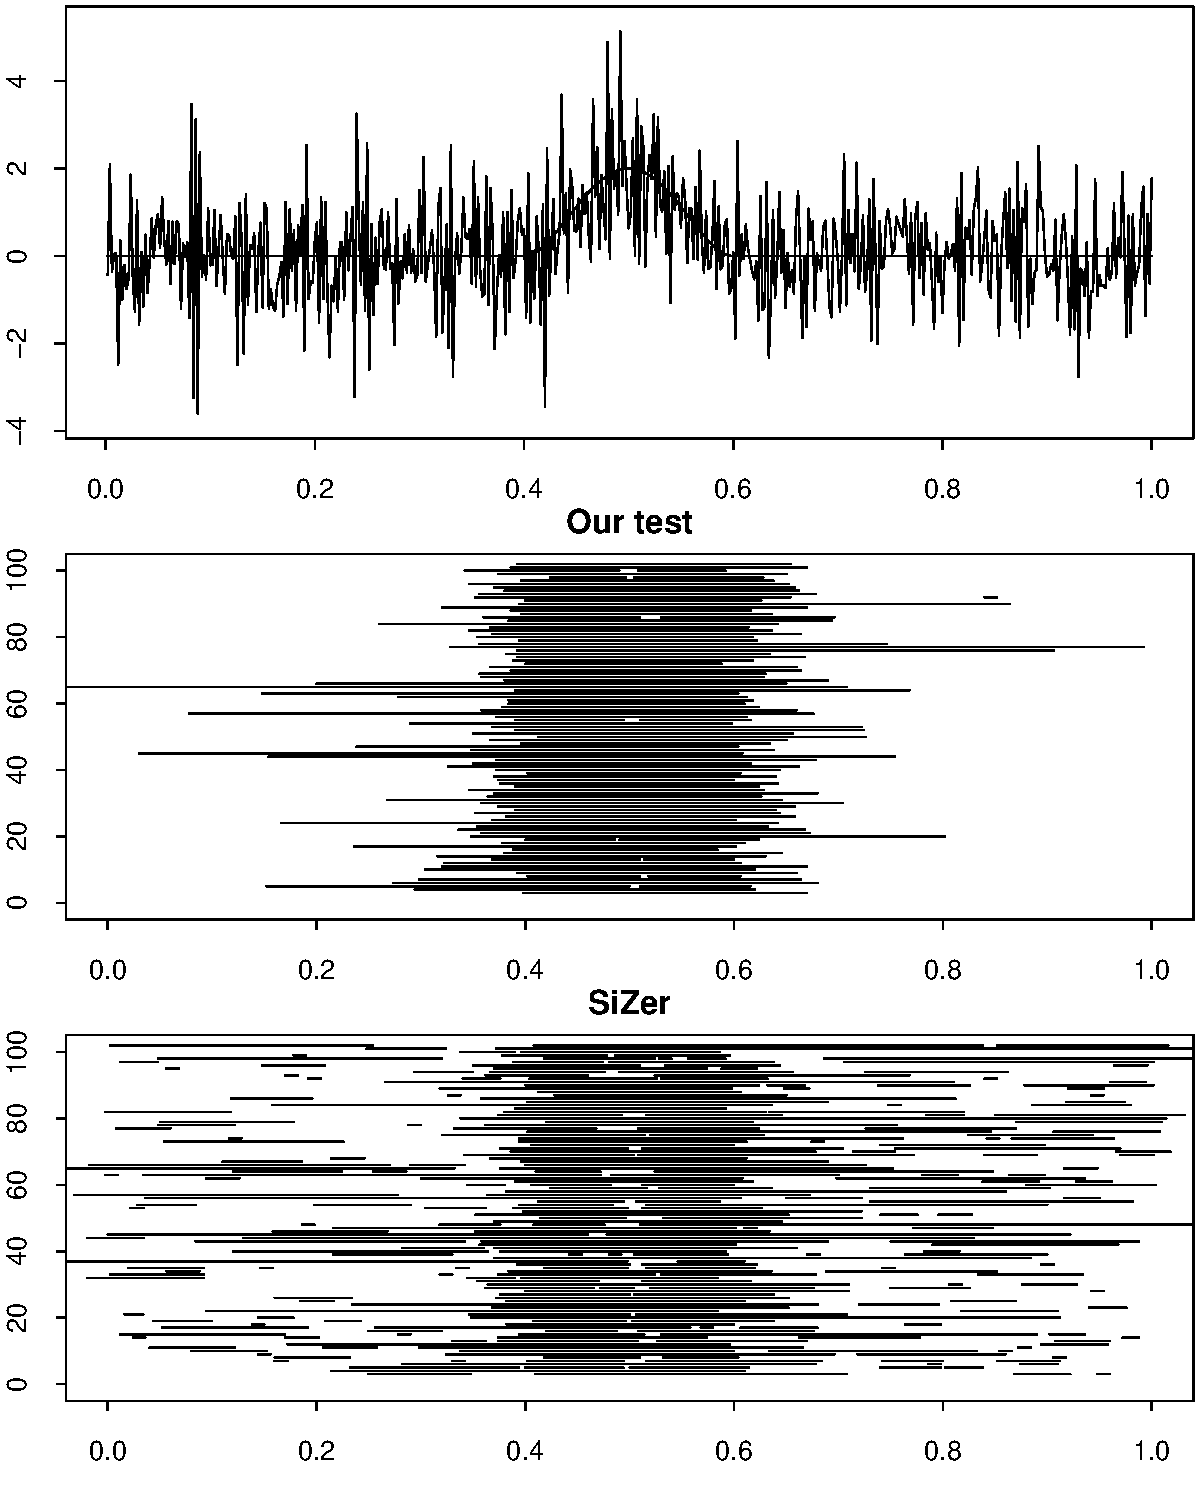
\includegraphics[width=.9\linewidth]{Plots/min_int_with_T_500_a1_-50.pdf}
%\caption{$a_1 = -0.5$}
%\end{subfigure}
%\begin{subfigure}{.5\textwidth}
%\centering
%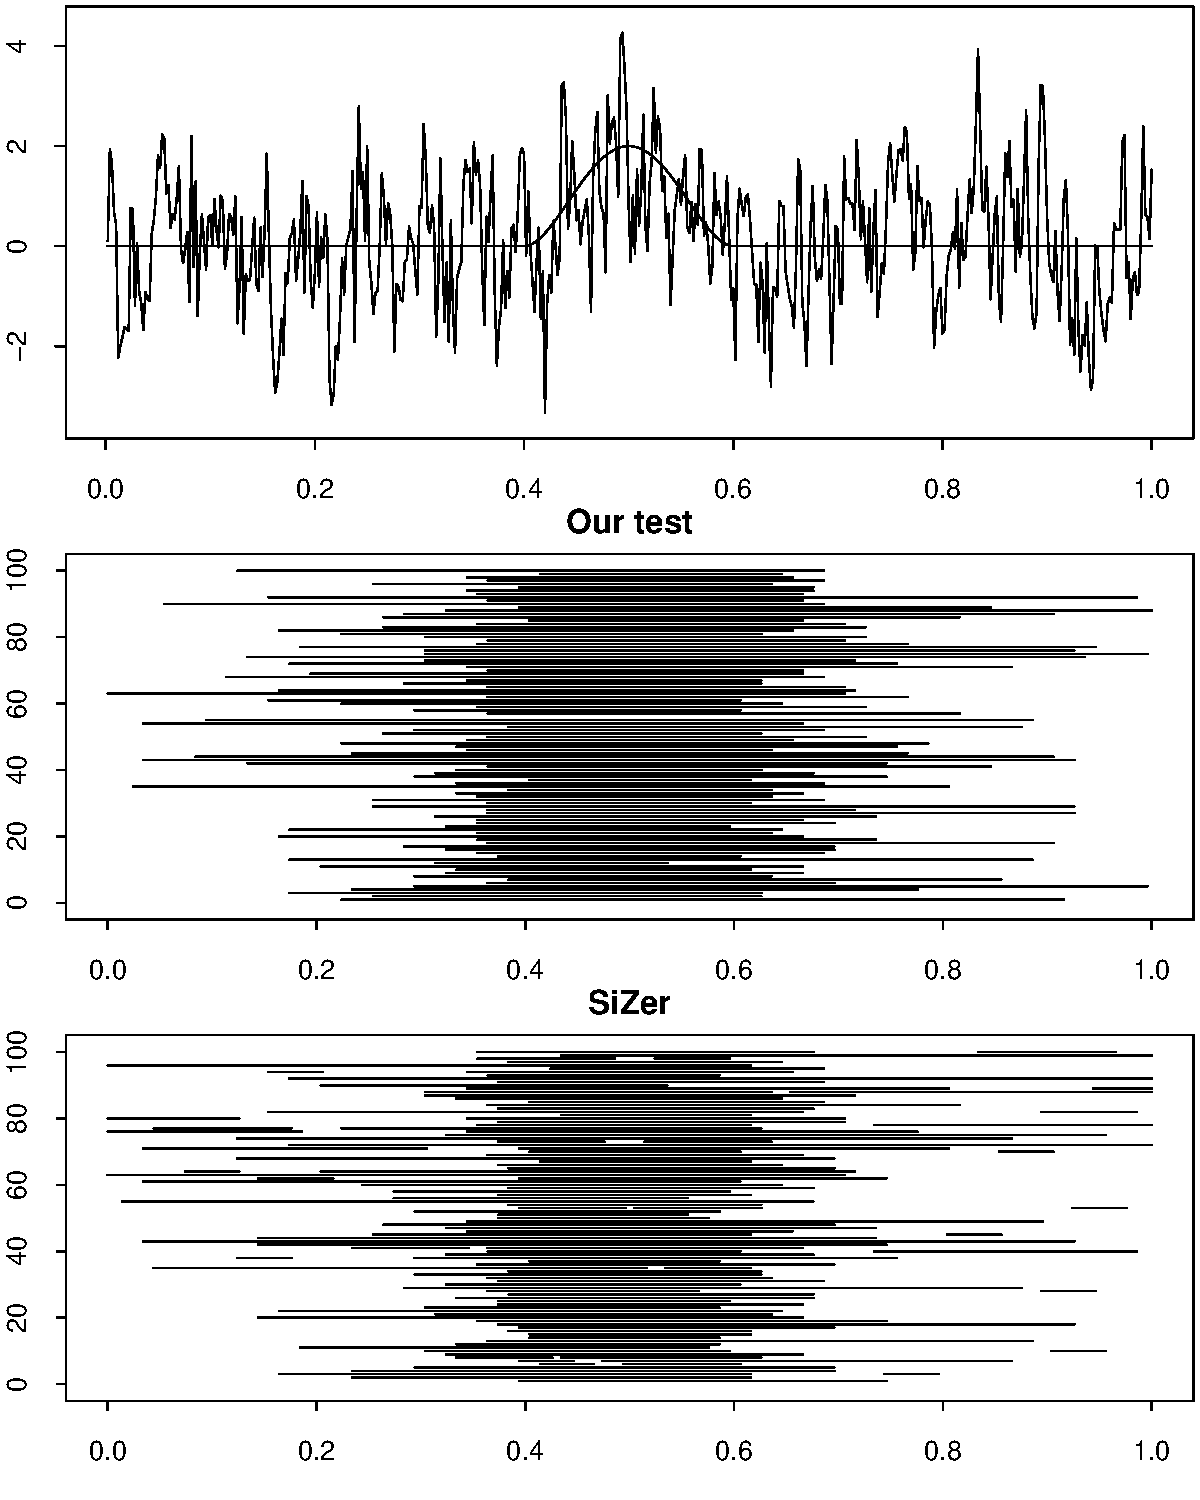
\includegraphics[width=.9\linewidth]{Plots/min_int_with_T_500_a1_50.pdf}
%\caption{$a_1 = 0.5$}
%\end{subfigure}
%\caption{Comparison of the regions $\mathcal{R}_T^\pm$ and $\mathcal{R}_T^{\text{SiZer}}$. Subfigure (a) corresponds to the model setting with the AR parameter $a_1 = -0.5$, subfigure (b) to the setting with $a_1 = 0.5$. The upper panel of each subfigure shows a simulated time series path together with the underlying trend function $m$. The middle panel depicts the regions $\mathcal{R}_T^\pm$ produced by our multiscale test for $100$ simulation runs. The lower panel presents the regions $\mathcal{R}_T^{\text{SiZer}}$ produced by SiZer.}  
%\label{fig:comparison_SiZer}
%\end{figure}

\begin{figure}[t]
\begin{subfigure}{.5\textwidth}
\centering
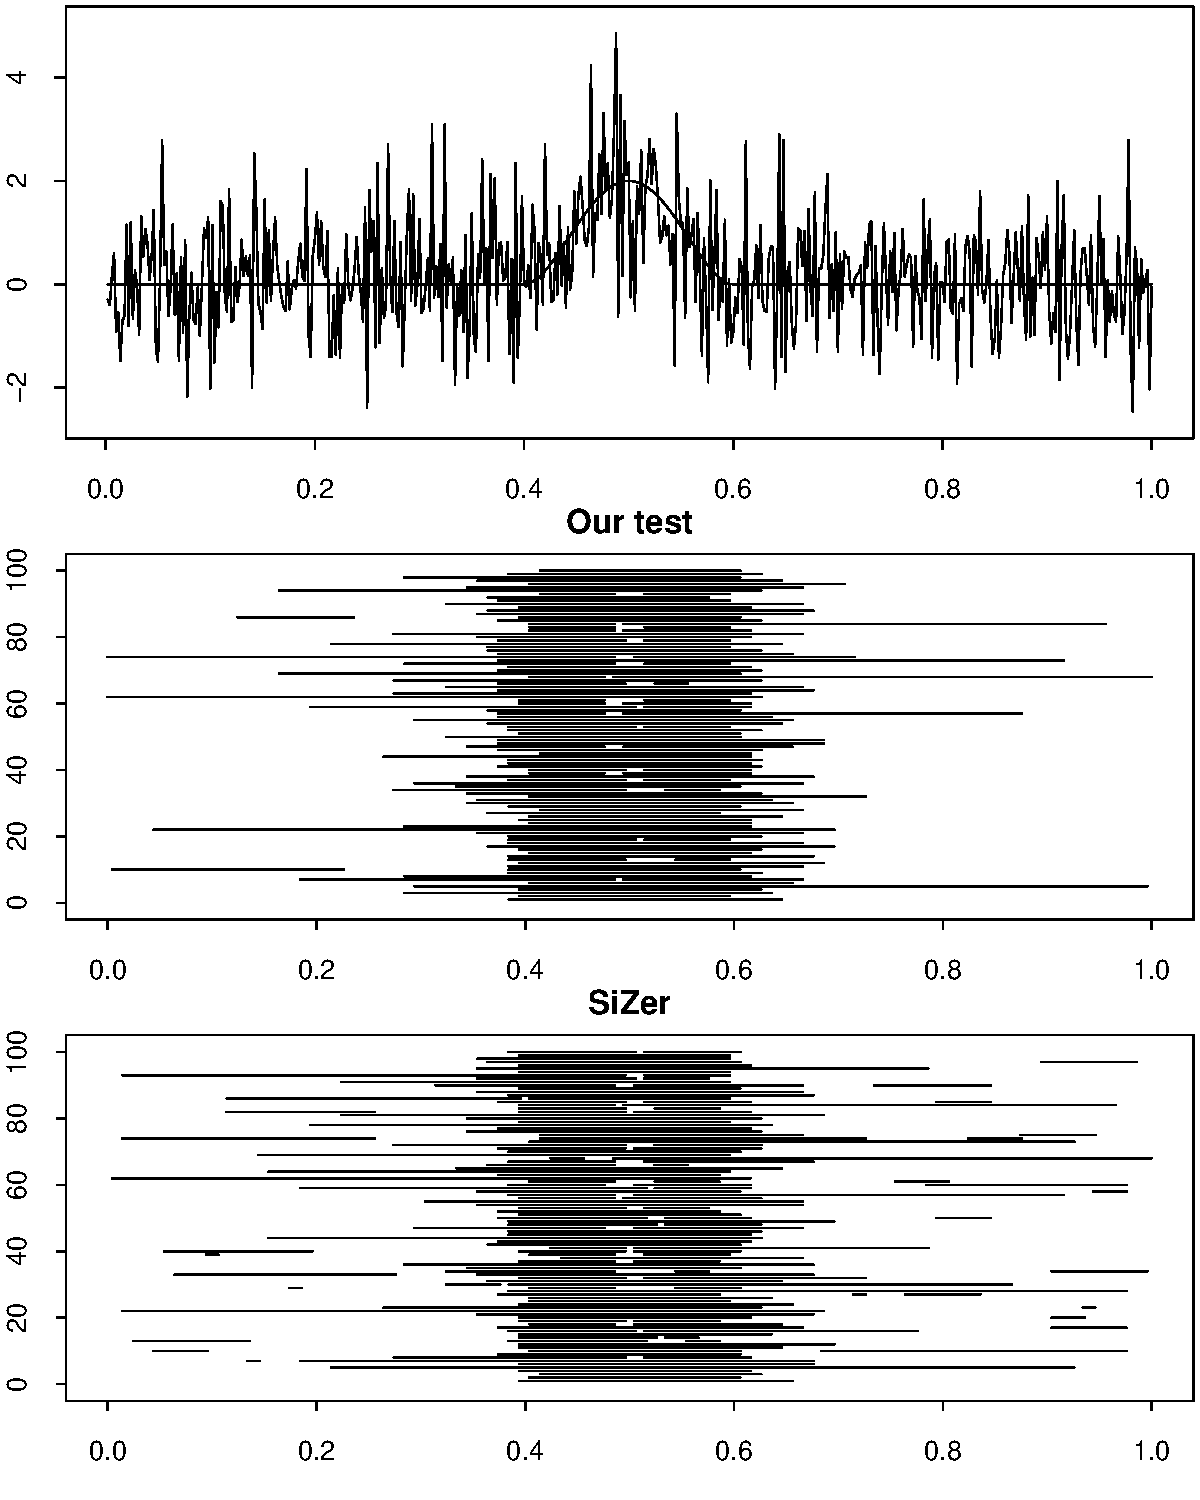
\includegraphics[width=.9\linewidth]{Plots/min_int_with_T_500_a1_-25.pdf}
\caption{$a_1 = -0.25$}
\end{subfigure}
\begin{subfigure}{.5\textwidth}
\centering
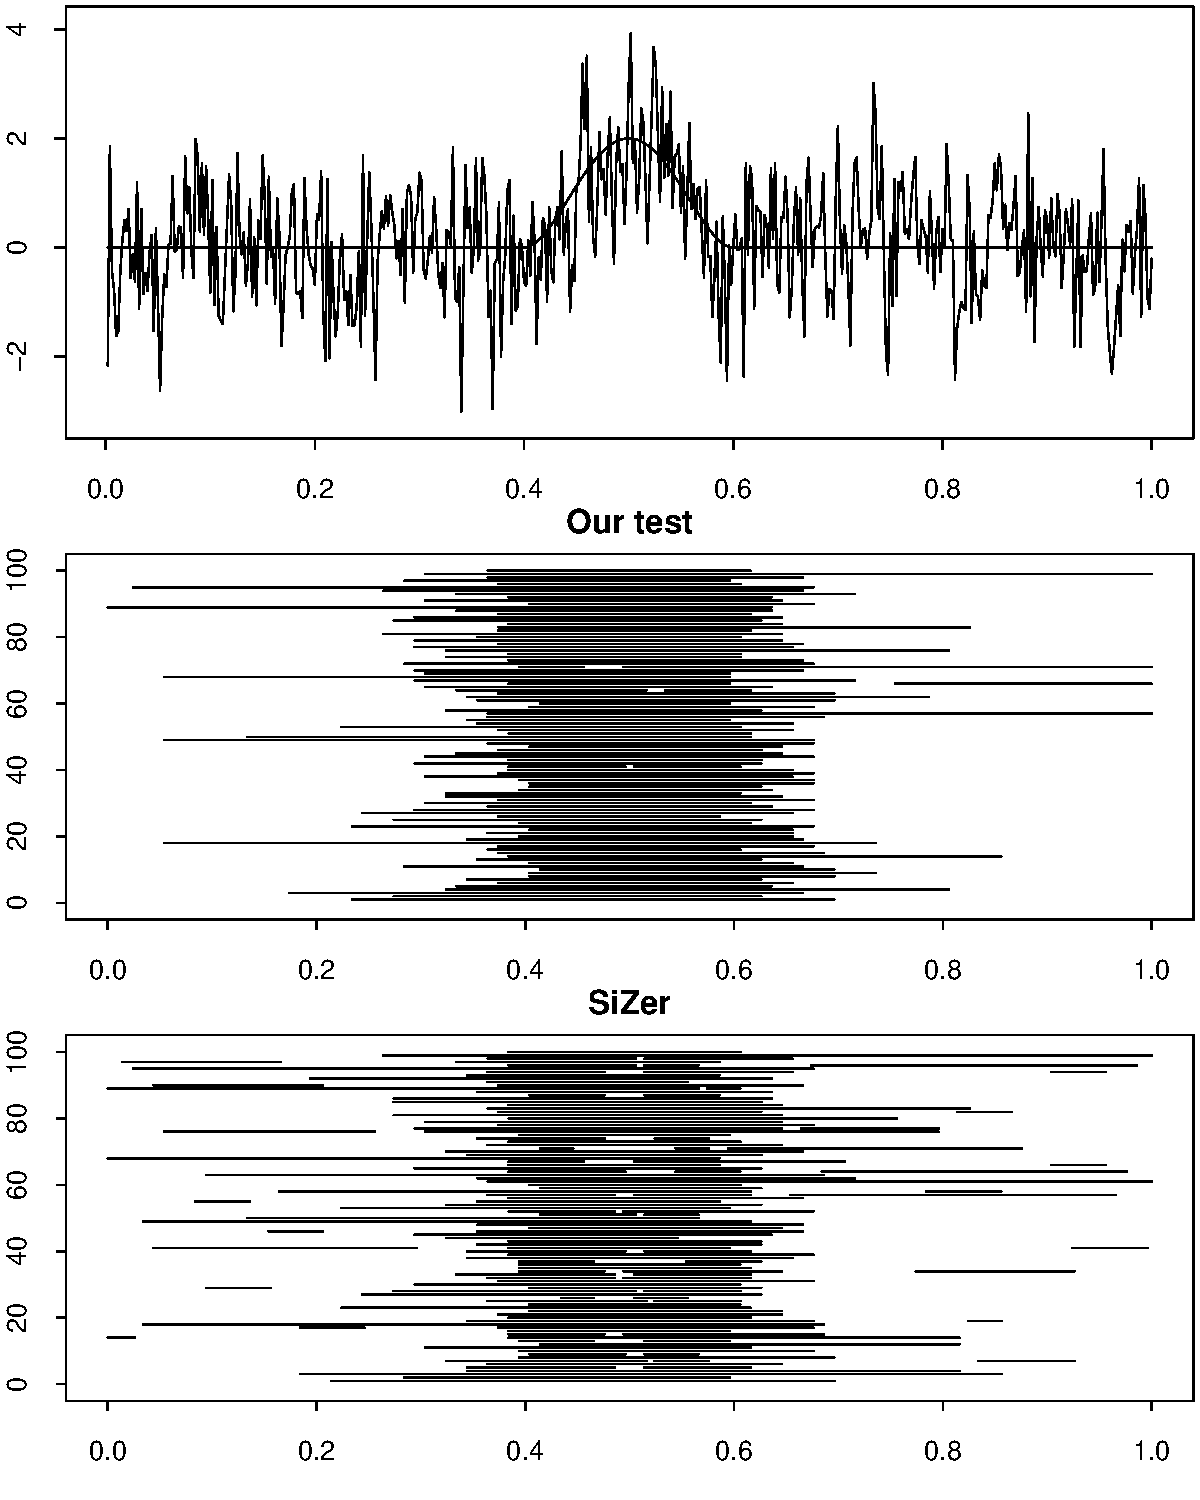
\includegraphics[width=.9\linewidth]{Plots/min_int_with_T_500_a1_25.pdf}
\caption{$a_1 = 0.25$}
\end{subfigure}
\caption{Comparison of the regions $\mathcal{R}_T^\pm$ and $\mathcal{R}_T^{\text{SiZer}}$. Subfigure (a) corresponds to the model setting with the AR parameter $a_1 = -0.25$, subfigure (b) to the setting with $a_1 = 0.25$. The upper panel of each subfigure shows a simulated time series path together with the underlying trend function $m$. The middle panel depicts the regions $\mathcal{R}_T^\pm$ produced by our multiscale test for $100$ simulation runs. The lower panel presents the regions $\mathcal{R}_T^{\text{SiZer}}$ produced by SiZer.}  
\label{fig:comparison_SiZer}
\end{figure}


We consider the same simulation setup as in the first part of the comparison study, only the trend function $m$ is different. We let $m$ be defined as $m(u) = 2 \cdot \ind(u \in [0.4,0.6]) \cdot (1 - 100 \{u-0.5\}^2)^2$, which implies that $\mathcal{R} = (0.4,0.5) \cup (0.5,0.6)$. The function $m$ is plotted in the two upper panels of Figure \ref{fig:comparison_SiZer}. We set the significance level to $\alpha= 0.05$ and the sample size to $T=500$. For each AR parameter $a_1 \in \{ -0.25,0.25 \}$, we simulate $S=100$ samples and compute $\mathcal{R}_T^\pm$ and $\mathcal{R}_T^{\text{SiZer}}$ for each sample. The simulation results are depicted in Figure \ref{fig:comparison_SiZer}, the two subfigures (a) and (b) corresponding to different AR parameters. The upper panel of each subfigure displays the time series path of a representative simulation together with the trend function $m$. The middle panel shows the regions $\mathcal{R}_T^\pm$ produced by our multiscale approach for the $100$ simulation runs: On the $y$-axis, the simulation runs $i$ are enumerated for $1 \le i \le 100$, and the black line at $y$-level $i$ represents $\mathcal{R}_T^\pm$ for the $i$-th simulation. Finally, the lower panel of each subfigure depicts the regions $\mathcal{R}_T^{\text{SiZer}}$ in an analogous way. 


Inspecting Figure \ref{fig:comparison_SiZer}, our multiscale method can be seen to approximate the region $\mathcal{R}$ fairly well in both simulation scenarios under consideration. In particular, $\mathcal{R}_T^\pm$ gives a good approximation to the region $\mathcal{R}$ for most simulations. Only in some simulation runs, $\mathcal{R}_T^\pm$ is too large compared to $\mathcal{R}$, which means that our method is not able to locate the region $\mathcal{R}$ sufficiently precisely. Overall, the SiZer method also produces quite satisfactory results. However, the SiZer estimates of $\mathcal{R}$ are not as precise as ours. In particular, SiZer spuriously finds regions of decrease/increase outside the interval $\mathcal{R}$ much more often than our method. It thus frequently mistakes fluctuations in the time series which are due to the dependence in the error terms for increases/decreases in the trend $m$. 

%For the negative AR parameter $a_1 = -0.25$, it performs substantially better than SiZer: For most simulations, $\mathcal{R}_T^\pm$ gives a good approximation to the region $\mathcal{R}$, whereas SiZer spuriously finds regions of decrease/increase outside the interval $\mathcal{R}$ quite often. SiZer thus frequently mistakes fluctuations in the time series which are due to the dependence in the error terms for increases/decreases in $m$. For the positive AR parameter $a_1 = 0.25$, the difference in performance is a bit less pronounced. Nevertheless, also here, SiZer spuriously detects increases/decreases in $m$ outside $\mathcal{R}$ much more often than our method. 


To sum up, our multiscale test exhibits good size and power properties in the simulations, and the minimal intervals produced by it identify the time regions where $m$ increases/decreases in a quite reliable way. SiZer performs clearly worse in these respects. Nevertheless, it may still produce informative SiZer plots. % (which is what it is designed for anyway). 
All in all, we would like to regard the two methods as complementary rather than direct competitors. SiZer is an explorative tool which aims to give an overview of the increases/decreases in $m$ by means of a SiZer plot. Our method, in contrast, is tailored to be a rigorous statistical test of the hypothesis $H_0$. In particular, it allows to make rigorous confidence statements about the time regions where the trend $m$ increases/decreases. %Such statements are not possible with SiZer. 

